\chapter{Discussion, future work \& conclusions}
\lhead{Chapter 5 \emph{Discussion, future work \& conclusions}}
\label{chap:5}
%\autoref{chap:5}

\bigskip
\section{Evaluation \& discussion}
\bigskip

In this section the experiments and results presented in the previous chapter will be evaluated. One way to assess the results of this software is to compare them with the equivalent information that has been published. For this reason, the results that were presented are concerning satellites or constellations that are well documented and information regarding the revisit time of them can be found.

To start with the experiments on the single satellites and as it can be seen in Figure \ref{revisit_time_Sentinel2A}, the average revisit time of Sentinel-2A at equator is almost 10 days, which can be confirmed from the official ESA's documentation \footnote{\label{Sentinel2_source}\textit{Available at: https://sentinel.esa.int/web/sentinel/missions/sentinel-2 (Accessed November 20, 2020)}}. Additionally, it can be noticed that there are certain longitude cells which the satellite does not pass. Since Sentinel-2A is in a Sun-synchronous orbit, it means that after a certain period of time the orbit repeats and it can also happen that the satellite never crosses some areas in the globe. The same characteristics and a revisit time of 10 days is also true for its twin satellite, Sentinel-2B.

\bigskip
In the same manner, the average revisit time of Sentinel-3A (Figure \ref{revisit_time_Sentinel3A}) is less than 2 days, which can be also validated \footnote{\label{Sentinel3A_source}\textit{Available at: https://sentinel.esa.int/web/sentinel/user-guides/sentinel-3-synergy/coverage (Accessed November 20, 2020)}}. The reason behind this rapid revisit time at the equator is the large swath width of its sensors, which is of 1270 km. This means that the larger the swath width of a sensor is, the larger is the area that is captured and thus the quicker the revisit time is.

It can be also noticed from the Figure \ref{revisit_time_Sentinel3A} that every longitude cell has information about the revisit time, which means that the satellite captures images along all the equatorial cells. On the one hand, this can be possibly explained by the fact that there is overlapping coverage between the adjacent orbits. For examining this case, the angular distance $\Delta \lambda$ of successive ascending equator crossings should be calculated (Equation \ref{delta_lambda}), once the period of the satellite has been found. So, for the Sentinel-3A the period is $T \sim 6056 \text{ [sec]}$ or $T \sim 101 \text{[ min]}$ and thus the $\Delta \lambda$ between the adjacent orbits is $\Delta \lambda \sim 25\text{ [degrees]}$. This can also be verified by plotting its groundtrack (see Figure \ref{Sentinel_3A_delta_lambda}). Finally, by converting the $\Delta \lambda$ from degrees to kilometers it is concluded that there is not overlapping coverage between the adjacent orbits, since the $\Delta \lambda \sim 2775\text{ [kilometers]}$ and swath width is 1270 km. All in all, in this revisit time calculation of Sentinel-3A it could be argued that even though there is not overlapping coverage between successive orbits as proved, the satellite is able to capture images along all the equatorial line. 

\begin{figure}
\centering
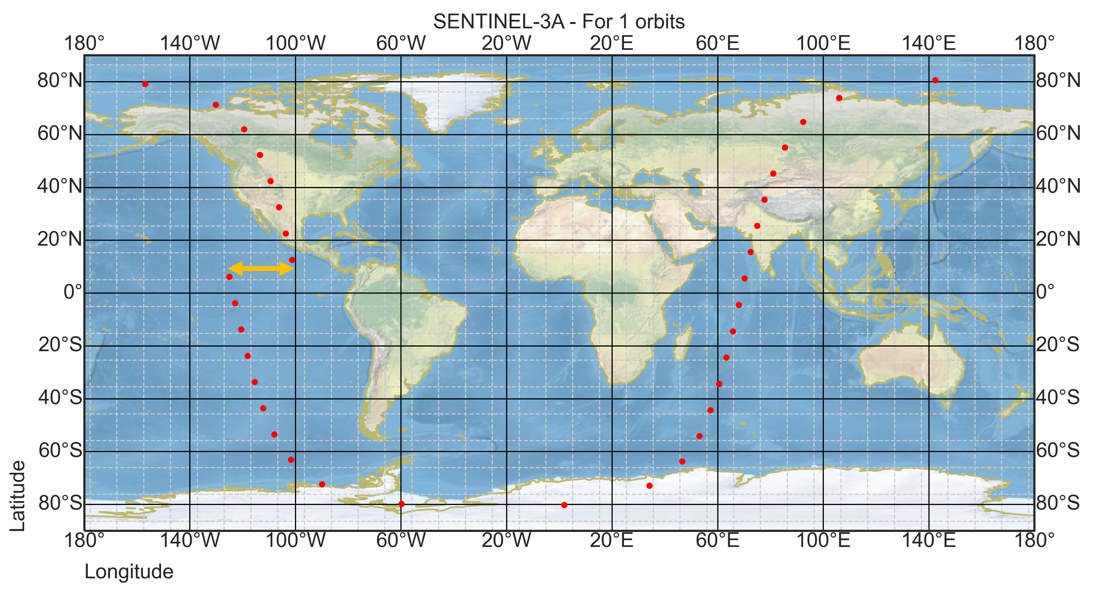
\includegraphics[width=0.9\textwidth]{Images/Sentinel_3A_delta_lambda.png}\caption{The groundtrack of Sentinel-3A for one orbit. The yellow arrow indicates the angular distance $\Delta \lambda$ of successive ascending equator crossings. As it can also be validated from the equation \ref{delta_lambda}, it is approximately 25 degrees.}
\label{Sentinel_3A_delta_lambda}
\end{figure}

\bigskip

The evaluation of the results of the two other presented single satellite's calculations of the revisit time along the equator comes from the JACIE's (Joint Agency Commercial Imagery Evaluation) group report of 2019 \cite{Christopherson}. To be more exact, in Figure \ref{revisit_time_of_ALSAT 1B} can be seen that the average revisit time at the equator is around 5 days, which can also be confirmed in the above-mentioned report. Similarly, the revisit time at the equator for the satellite GOMX-4A has been also found to be 5 days.

\bigskip
As for the evaluation concerning the revisit time of multiple satellites or constellations, it was first important to make sure that all the involved satellites have the same starting epoch for their propagation. For this reason, the groundtrack of one orbit for the Sentinel-2 constellation was presented. In Figures \ref{groundtrack_Sentinel-2A}, 
\ref{groundtrack_Sentinel-2B} it can also be verified the fact that those twin satellites are phased at 180 degrees to each other.

The average revisit time at the equator for the Sentinel-2 constellation is around 5 days, as it can be seen in Figure \ref{revisit_time_of_SENTINEL-2A_SENTINEL-2B}, which can be validated by ESA's documentation \footnote{\label{Sentinel2_source}\textit{Available at: https://sentinel.esa.int/web/sentinel/missions/sentinel-2 (Accessed November 20, 2020)}}. Similarly, the revisit time for the Sentinel-1 constellation is 3 days as seen in Figure \ref{revisit_time_of_SENTINEL-1A_SENTINEL-1B}, whose validity can be also checked \footnote{\label{Sentinel1_source}\textit{Available at: https://sentinel.esa.int/web/sentinel/user-guides/sentinel-1-sar/revisit-and-coverage (Accessed November 20, 2020)}}.

\bigskip
Regarding the first experiment of finding the position of a new satellite, which can achieve a more frequent revisit time together with a group of other satellites, namely the Sentinel-2 constellation, the Figure \ref{revisit_time_ofdoubleaxis_SENTINEL-2A_SENTINEL-2B_Example-satellite} was created. As can be seen, the overall revisit time of the three satellites was calculated also at the positions of Sentinel-2A and 2B individually. For those positions, indicated with green lines, the overall revisit time was found to be close to 5 days. The reason behind is that the Example-satellite in these positions is co-located with one of the two other satellites, which fact does not result in reducing the revisit time of the one achieved only by the Sentinel-2 constellation. The revisit time of 5 days in those positions can also be validated from the Figure \ref{revisit_time_of_SENTINEL-2A_SENTINEL-2B}, in which the average revisit time at equator of the Sentinel-2 satellites is shown.

Additionally, it was noticed that although the influence of the new satellite's mean anomaly change in the combined revisit time brings a large reduction rate, of about 35\%, the differences of the revisit time between the various positions in the orbital plane are not large (Figure \ref{revisit_time_ofdoubleaxis_SENTINEL-2A_SENTINEL-2B_Example-satellite}). Therefore, placing a new satellite in the same orbital plane as of the other satellites will bring a significant reduction in the revisit rate independently of the exact position in the orbital plane. %Nevertheless, attention needs to be paid to not placing a new satellite in the same position as another existing satellite is.
%Which, in practice, would also not be done, as no one wants to deal with the permanent collision risk ;-) 

\bigskip
The second experiment pertained to the investigation of the overall revisit time when the altitude of the new satellite varies. For this case, several examples were presented in Chapter \ref{chap:4} and in each of those the new satellite is placed in a different position in the orbital plane. More specifically, as can be seen in Figures \ref{revisit_time_ofdoubleaxisaltitude_SENTINEL-2A_SENTINEL-2B_Example-satellite_50deg}, \ref{revisit_time_ofdoubleaxisaltitude_SENTINEL-2A_SENTINEL-2B_Example-satellite_180deg}, \ref{revisit_time_ofdoubleaxisaltitude_SENTINEL-2A_SENTINEL-2B_Example-satellite_330deg}, in all those example cases the same behavior can be noticed. The most frequent revisit time is close to the altitude that the rest of the satellites are located and the revisit time becomes less often the further away the satellite is located from this altitude. As for the reduction of the revisit time that can be seen in the right-side y-axis of the Figures, it should be mentioned that is the same compared with the reduction rates from the previous experiment when varying the position in the orbital plane.
% The influence of the altitude change in the revisit time is that it is always drifting with respect to the other. --> THE MORE YOU GO AWAY FROM THAT ALTITUDE, THE LESS PRONOUNCED WILL BE THE DIFFERENCE COMPARED TO THE DIFFERENCES FROM THE MEAN ANOMALY'S CASE.

The same experiment of varying the altitude of a new satellite when it is added in the calculation of the overall revisit time was implemented for the group of the 37 Flock-3P satellites (Figure \ref{revisit_time_ofdoubleaxisaltitude_Flocks}). As mentioned above, the revisit time is drifting with respect to the altitude change, with the lowest point being in the mean altitude of the rest of the satellites. Despite that, in this case in which the number of engaged satellites is as large as of 37, the reduction of the revisit time as can be seen in Figure, is around $2-3\%$. In comparison with the reduction of the revisit time when a satellite is added to a smaller group of satellites ($\sim 34\%$ e.g. Figure \ref{revisit_time_ofdoubleaxisaltitude_SENTINEL-2A_SENTINEL-2B_Example-satellite_50deg}), this rate is significantly lower, which indicates that by adding one satellite in an already large group of satellites does not contribute much in the accomplishment of a rapider revisit time.

\bigskip
Last but not least, the final experiment is inspired by the recent announcement of \textit{Planet}, promising that any part of the world will be revisited every two to four hours and for this reason more satellites added to the Skysat fleet will be launched \footnote{\label{Flock_source}\textit{Available at: https://spacenews.com/planet-explore-2020/ (Accessed November 20, 2020)}}. That being said, in this experiment the entire Flock constellation was used in order to find out whether there are already operational and orbiting satellites which can achieve these revisit rates. In fact, the average revisit time at equator for those 155 satellites of the Flock constellation is approximately four hours, a revisit rate close to the desired one.

From this experiment, it can be seen how dozens of new satellites are launched in order to contribute to achieving a certain revisit rate, which can be already accomplished by an operational constellation. Thus, the importance of the creation of space traffic management rules based on the added value that each new satellite may have, needs to be underlined.
% Combination of all Flocks (not even Skysats) and the revisit time close.. imagine that since the calculation is at equator and the orbits are near-polar, at the equator is the less frequent revisit time.


%$The discussion will consist of argumentation. In other words, you investigate a phenomenon from several different perspectives. To discuss means to question your findings, and to consider different interpretations. Here are a few examples of formulations that signal argumentation:
%
%On the one hand … and on the other …
%However …
%… it could also be argued that …
%… another possible explanation may be …


\bigskip
\subsection{Strengths \& contribution of thesis}
\bigskip

Along with the completion of this work, a review and evaluation of the strengths of it was conducted. One contribution that this thesis has offered is the fact that a clear definition and way of computing the revisit time was given. The importance of this contribution is that all the information regarding the revisit time of satellites announced by renowned companies is vague, since the assumptions and methods that were made in order to compute this information are unknown.

However, there are companies, such as \textit{Planet}, which announce a revisit time of a constellation measured from a reference altitude, which is not in line with the actual altitude of the satellites of this constellation. As an example, the Skysat constellation is mentioned to achieve revisit time of four to five days, in a reference altitude of 500km \footnote{\label{Planet_skysat}\textit{Source: https://assets.planet.com/docs/Planet_Combined_Imagery_Product_Specs_letter_screen.pdf (Accessed December, 2020)}}. However, the mean altitude of the constellation is around 350-450 km and results in approximately seven days of revisit time. The fact that the revisit time is calculated for such an altitude reference might also serve as a marketing strategy of attracting more customers since the revisit time is more frequent than the one acquired from the actual satellite's altitudes. 

Having said that, a user has the possibility of finding out the revisit time of not only single satellites, but the overall revisit time of constellations or group of satellites, which information is difficult to be found elsewhere pre-calculated. Another feature that this software offers is that the latitude of interest to the user can be selected in order to compute the revisit time there, together with the default approach of calculating it at the equator.

It was also proved by the demonstrated experiments in the Chapter \ref{chap:4} that the software in tandem with the database can reveal information related to the added value of a future satellite based on how many other similar objects offer a certain service already. Thus, this thesis has contributing into the field of prioritizing the missions based on the added value to the society.


% Revisit time VS repeat period. 1st overlapping gaps + swath width (characteristic of sensor) --> Importance of applications -- Questions might arise.

\bigskip
\subsection{Limitations} %Problems
\bigskip

The main input of this application, but also a source that can affect the performance of the software is the time of reference and the accuracy of the TLE of the satellites. Firstly it needs to be mentioned that the orbital elements of the satellites go rapidly out of date. This means that the \textit{epoch} of the TLE set should be in a recent date, for the reason that the older it is, the more inaccurate the parameters might be. In particular, since the application targets to the future states of the satellites when computing the added value of a future satellite or the overall revisit time of a satellite added to a group of satellites, it is necessary to have the most recent TLE. Fortunately, the providers, such as \textit{CelesTrak} or \textit{Space-track.org}, update them almost daily for satellites in LEO, which fact can give a solution to this problem.
%A TLE set can predict the position of a satellite approximately for  two weeks into the future.

However, the exact process for updating TLE is not well known with every detail. Essentially, observations are collected several times a day at the 18\textsuperscript{th} Space Control Squadron (18 SPCS) operated by the US Air Force Space Command (AFSPC).
Then, the satellite observation processes are executed in an automated way. At first, an initial association and verification pass is executed in order to be passed to the orbit determination (OD) operation. Whether a satellite from the observed ones had to be maneuvered in a temporary orbit is not known. Thus, in case there are maneuvers, the corresponding TLE sets of those satellites have large errors \cite{TLE_Vallado}. This finally affects to the results of the current software, since it receives as input those TLE sets. Reassuringly, in the Section \ref{Future work}, a way of investigating whether a TLE set of a satellite belongs to orbit of a maneuvered satellite is suggested. 

%Once, the observation pass through an initial association and verification pass, they are passed to the orbit determination operation using SGP4 and numerical techniques (cite: TLE_Vallado)
%There is no knowledge of maneuvers before or after the current time of OD generation. During the processing, the presence of maneuvers inflates the uncertainty of any estimate, but because the TLEs are delivered without a covariance, there is little way of knowing if there is increased uncertainty in a particular TLE from the previous estimates. Indeed as it was investigated by Intelsat, The JSPOC has no knowledge of the satellite owner maneuvers and naturally the TLE of the maneuvering satellites have large errors. (cite: TLE_Vallado)
% Another issue that arises with the TLE's use is (maybe shift this first). "It should be noted that when using TLE sets from NORAD, it is important to realize that not just any prediction model can be used. The elements of NORAD TLEs are mean values, which were obtained by removing periodic variations in a particular way (SGP4 way). To get the most precise prediction results it is important that these variations will be reconstructed in the same way as they were removed. When the SGP4 model is used, these optimal results are achieved. However, in this application, since high precision is not necessary... It general periodical SGP model gives approximately 1 km accuracy over a short (ca few days) propagation time. (VALLADO)

\bigskip
At last, the presence of a few outliers in the results of the revisit time of entire constellations needs to be mentioned. For this reason, the assumptions and simplifications that were made in the process of producing the results, should be selected more carefully. As an example, the simplification of calculating the revisit time taking as swath width the larger of the available ones, might lead to inconsistent results between the satellites of a constellation (see Section \ref{how_to}). One parameter, which might also be the source of outliers, is the likelihood of incorrect TLE sets, which may correspond to the position of a maneuvered satellite as it was previously mentioned. Finally, it needs to be highlighted that the duration of the simulations was selected to be approximately 20 days, which is translated as 300 orbits in the case of the LEO satellites that were part of the above experiments (see beginning of Chapter \ref{chap:4}). All the same, in case of satellites orbiting in higher altitudes this assumption needs to be modified and selected appropriately.

% Maybe add sth about the duration of the simulations.. about the resonance?! (I had written some stuff at the beginning of the 4th Chapter) "Some satellites hit resonances. Needs more careful investigation.. Some satellites have longer revisit time than others (from the same constellation). I am not sure if I want to say this :) Or mention that their results might belong to maneuvered satellites...


\bigskip
\section{Future work}
\label{Future work}
\bigskip

During the implementation of this thesis, the areas of its further improvement were discovered. However, due to time and resources limitations, these areas may suggest future work.

One direction of future work is the modification of the software in order to be applicable to satellites from other fields apart from EO, such as Communication. That being the case, the software needs to be expanded in calculating the revisit time from all types of inclined orbits; from low inclination to near-polar ones. To be more specific, the calculation of the coverage along the equator needs to be modified in respect to the inclination angle and the swath width (see Figure \ref{swath_width_groundtrack}).

\bigskip
Furthermore and apropos the main limitation of thesis, several steps can be implemented in order to reduce the likelihood of using an outdated or inaccurate TLE set. Firstly, the database can be connected to a TLE provider. In this way the orbital elements of each satellite can be automatically updated, while preserving the information related to the characteristics of the EO sensors.

In addition, in order to detect whether each and every TLE set provides the application with a satellite's position during an orbital maneuver or not, the method of Lemmens and Krag [2014] can be used. This is achieved by checking the consistency between arbitrary TLE sets of the same object \cite{Lemmens}. Then, not only the non-natural anomalous and unexpected events of orbits can be found, but also the TLE set that produced this kind of orbit can be left out from the further calculations until is discovered whether this new presented orbit is a permanent one.

At last, for reducing the computational times needed for providing the information of revisit time to the user, parallel computing methods can be used. Then, by increasing the number of computations, which can be performed in a given period of time, the outcome is calculated faster.

% % Info about the tilt angle -- I had mentioned somewhere in the thesis, that if this information exists, then the revisit time is calculated based on it. So... do not mention it now.
% % Calculation of revisit time metrics considering time of night/day or lighting conditions would also enable particular application for optical Earth observation sensors. (mallon min to anafereis. Einai polu sxetiko me tin ergasia... Mipos na to eixa kanei?)
% % what can be done more? Finally, more complex sensor shapes could be investigated and different projection geometries could be studied to ensure accuracy of the method at higher target latitudes.
% Place an index at the "international designator" in the PostgreSQL for faster searching. So far is not needed.

\bigskip
\section{Conclusions}
\bigskip

From the presented experiments it can be deduced that the rapider revisit rates can be achieved when adding a satellite in the same orbital altitude and not placing it in a higher or lower one. However, if the orbital plane has already a large number of satellites, then the option of changing the altitude of the new satellite is inevitable in order to avoid the risk of conjunctions between the other satellites. All the same, in such case the altitude change of the new satellite should not exceed five km above or below the altitude of the main's orbital plane, since the further away from the initial altitude the satellite goes, the less frequent the revisit times become.

Moreover, the addition of a single satellite to an already large constellation does not result in a significant reduction of the revisit time. From the experiment of the whole Flock constellation, it can be assumed that the revisit rates that a company aims to achieve by launching a new constellation or satellites, can be achieved by operational and orbiting satellites collaboratively. As proved in the previous Chapter, this software can perform such investigations.

\bigskip
All in all, the objectives of this thesis were met, since a software was developed, with which useful information can be gained towards the prioritization of missions based on the added value in the society. As an example, it can be suggested that the satellites, which can achieve a significant increase of the revisit rate, have a higher added value compared to other satellites or mission, which do not come with any considerable changes.

In this way, this work can give the incentives so that space traffic management rules to be created and cooperation between different entities to be actualized. Additionally, the produced results from the application regarding the revisit time of a single or multiple satellites can also potentially provide valuable reference for the Earth observation system designers in the early phases of a mission development cycle.
%Who will be helped with this work? It will give the incentives etc etc buuuut These plots on their own and the supporting data can provide valuable reference for Earth observation system designers in the early phases of a mission development lifecycle. (By Crisp_2018 p.10) 


% Check comments on "Scientific questions.doc" (about revisit time, inclination, swath width, altitude etc)
% First, the revisit time is latitude dependent! Since we find the revisit time at the equator and we have near-polar orbits, the equator has the less frequent revisit time.